\chapter{CADRE THÉORIQUE DU CDPR}

\section{Principes}

Un robot parallèle à câbles se distingue des manipulateurs classiques par une contrainte physique simple : un câble ne peut que tirer, jamais pousser. Cette particularité redéfinit entièrement la façon de modéliser le système, depuis la géométrie de sa plateforme jusqu'aux limites de l'espace dans lequel il peut réellement se déplacer.

\subsection{Comparatif des architectures robotiques}

En robotique, on distingue deux grandes familles de manipulateurs selon la manière dont l'effecteur est relié au bâti. Un robot série relie sa base à son effecteur par une seule chaîne cinématique, articulation après articulation, comme un bras manipulateur industriel classique. Un robot parallèle, lui, relie l'effecteur au bâti par plusieurs chaînes cinématiques indépendantes fonctionnant en même temps. Cette architecture améliore généralement la rigidité et la capacité de charge, mais réduit souvent l'espace de travail et complexifie les modèles géométriques.

Le robot parallèle à câbles (\textit{Cable-Driven Parallel Robot}, CDPR) est un cas particulier de robot parallèle dans lequel les liaisons rigides sont remplacées par des câbles. Sa plateforme mobile est suspendue et actionnée par un ensemble de câbles reliés à des enrouleurs motorisés fixés sur une structure porteuse \cite{dahiya2022}. Dans les architectures dites sur-contraintes, les câbles ne peuvent que tirer, jamais pousser, c'est ce qui distingue fondamentalement les CDPR des robots parallèles classiques à liaisons rigides. Ces robots se caractérisent en particulier par un grand espace de travail et des accélérations élevées, grâce à leur faible inertie comparée aux manipulateurs série ou parallèles classiques.

La littérature emploie parfois des termes équivalents comme \textit{cable-driven parallel manipulator} (CDPM) ou simplement \textit{cable robot} (CR) ; le sigle CDPR sera utilisé de façon exclusive dans ce mémoire.

\begin{figure}[H]
\centering
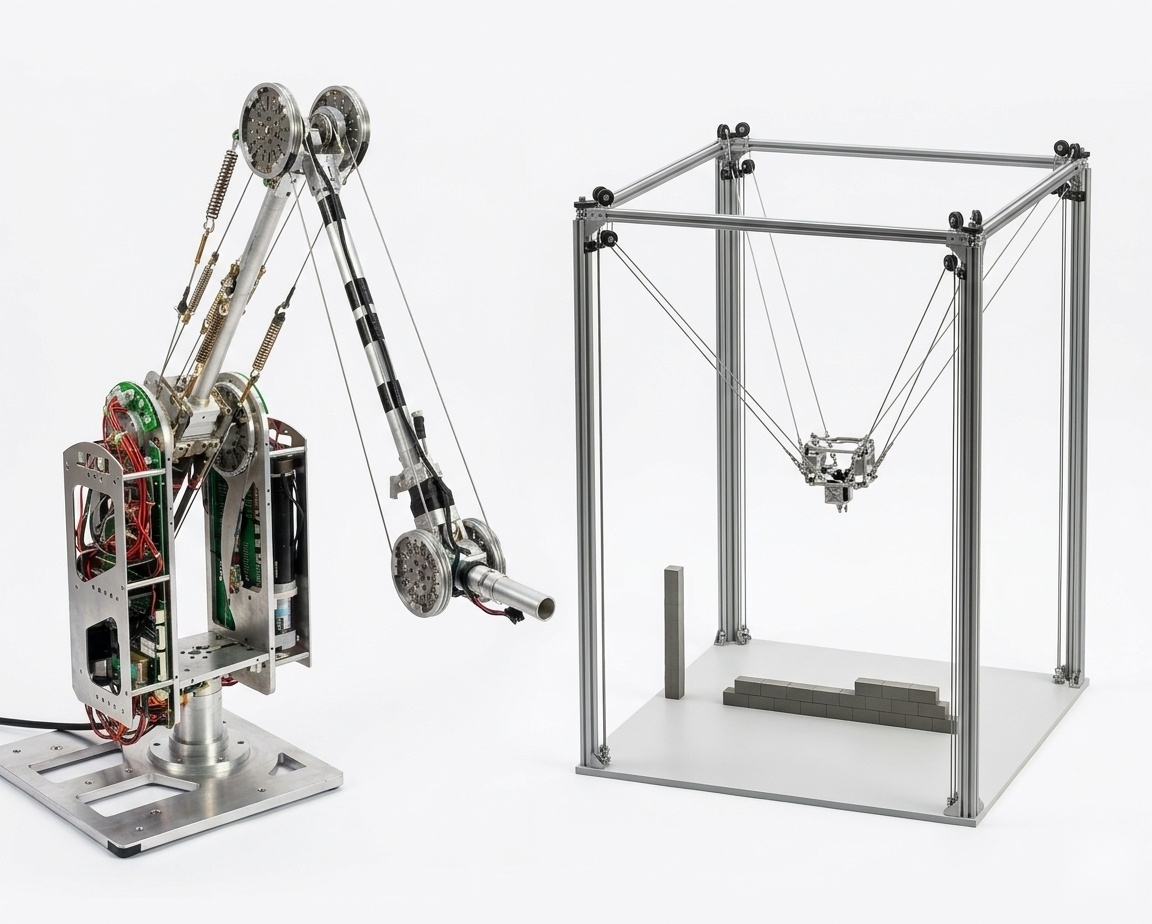
\includegraphics[width=0.88\textwidth]{robots_serie_parallele.jpg}
\caption{Robot série et robot parallèle à câble}
\label{fig:serie_parallele}
\end{figure}

\subsection{Terminologie CDPR}

Un CDPR se compose classiquement des éléments suivants :

\begin{table}[H]
\centering
\caption{Cadre théorique d'un CDPR}
\label{tab:terminologie}
\begin{tabular}{|>{\raggedright\arraybackslash}p{4.0cm}|>{\raggedright\arraybackslash}p{10.8cm}|}
\hline
\textbf{Terme} & \textbf{Définition} \\
\hline
Structure porteuse / bâti fixe & Cadre fixe sur lequel sont montés les enrouleurs. \\
\hline
Enrouleur & Dispositif motorisé qui enroule ou déroule le câble pour en faire varier la longueur active. \\
\hline
Point d'ancrage & Point, côté bâti ou côté plateforme, où le câble est guidé ou fixé. \\
\hline
Plateforme mobile (PM) & Organe terminal suspendu par les câbles, dont la pose est déterminée par le contrôle coordonné des longueurs de câble. \\
\hline
Reconfigurable & Capacité à modifier la géométrie du robot en déplaçant les points d'ancrage, sans changer la structure porteuse. \\
\hline
Degré de liberté (DDL) & Nombre de paramètres indépendants nécessaires pour décrire la pose de la plateforme (jusqu'à 6 en 3D : 3 translations + 3 rotations). \\
\hline
\end{tabular}
\end{table}

\begin{figure}[H]
\centering
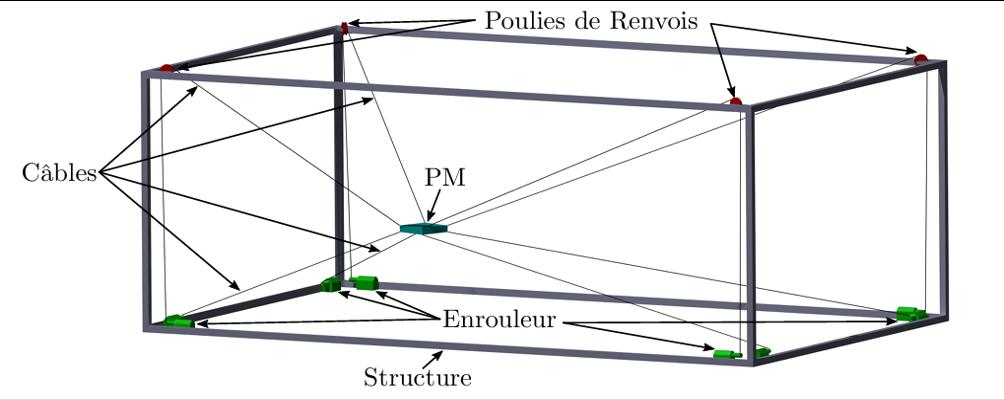
\includegraphics[width=0.92\textwidth]{cdpr_annote.png}
\caption{Schéma annoté d'un CDPR}
\label{fig:cdpr}
\end{figure}

\subsection{Classification cinématique}

Le critère de classification le plus fondamental des CDPR compare le nombre de câbles actifs \( m \) au nombre de degrés de liberté \( n \) de la plateforme :

\begin{itemize}[itemsep=3pt]
  \item \textbf{Sous-contraint} (\( m < n+1 \)) : les câbles ne suffisent pas à contraindre tous les mouvements possibles ; l'équilibre nécessite l'aide de la gravité ou d'une force extérieure.
  \item \textbf{Totalement contraint} (\( m = n+1 \)) : les câbles suffisent tout juste à contraindre tous les degrés de liberté.
  \item \textbf{Sur-contraint / redondant} (\( m > n+1 \)) : le nombre de câbles dépasse le strict nécessaire, ce qui améliore la capacité à générer des efforts dans toutes les directions, mais impose de répartir la tension entre câbles, car plusieurs répartitions sont possibles pour une même pose.
\end{itemize}

Une seconde classification distingue les CDPR selon la disposition des câbles par rapport à la plateforme :

\begin{itemize}[itemsep=3pt]
  \item \textbf{Architecture suspendue} : tous les câbles sont positionnés au-dessus de la plateforme ; la gravité maintient les câbles en tension. L'espace sous la plateforme reste dégagé, ce qui favorise un grand espace de travail, au prix d'un fonctionnement plutôt statique.
  \item \textbf{Architecture à câbles antagonistes} : les câbles sont répartis de part et d'autre de la plateforme et tirent les uns contre les autres, garantissant des tensions positives indépendamment de la gravité, ce qui permet des mouvements plus dynamiques.
\end{itemize}

\section{Modèles géométriques}

\subsection{Modèle géométrique inverse (MGI)}

Le MGI répond à une question simple : quelle longueur de câble faut-il pour amener la plateforme dans une pose donnée ? Pour un robot à câbles, ce problème se ramène en réalité à un calcul de distance entre deux points, ce qui en fait le plus facile à résoudre des trois modèles.

Notons $m$ le nombre de câbles, $(\mathbf{a}_i)$ le point d'ancrage fixe du câble $i$ sur le bâti, $(\mathbf{b}_i)$ son point d'attache sur la plateforme (exprimé dans le repère corps), $(\mathbf{p} = [x,y,z]^T)$ la position du centre de la plateforme dans le repère monde, et $(\mathbf{R})$ la matrice de rotation associée. Le vecteur reliant l'attache à l'ancrage s'écrit :
\begin{equation}
\mathbf{q}_i = \mathbf{a}_i - \mathbf{p} - \mathbf{R}\mathbf{b}_i
\label{eq:qi}
\end{equation}
D'où la longueur du câble $i$, simple norme de ce vecteur :
\begin{equation}
l_i = \|\mathbf{q}_i\| = \|\mathbf{a}_i - \mathbf{p} - \mathbf{R}\mathbf{b}_i\|
\label{eq:li}
\end{equation}

\paragraph{Translation et rotation autour de Z.}
Dans cette configuration, la plateforme possède quatre degrés de liberté : les trois translations $(x, y, z)$ et une rotation $(\varphi)$ autour de l'axe vertical. La matrice de rotation prend la forme :
\begin{equation}
\mathbf{R}(\varphi) = \begin{pmatrix}
\cos\varphi & -\sin\varphi & 0 \\
\sin\varphi & \cos\varphi & 0 \\
0 & 0 & 1
\end{pmatrix}
\label{eq:Rphi}
\end{equation}
Pour un point d'attache $(\mathbf{b}_i = [b_{ix}, b_{iy}, b_{iz}]^T)$, on obtient :
\begin{equation}
\mathbf{R}(\varphi)\mathbf{b}_i = \begin{pmatrix}
b_{ix}\cos\varphi - b_{iy}\sin\varphi \\
b_{ix}\sin\varphi + b_{iy}\cos\varphi \\
b_{iz}
\end{pmatrix}
\end{equation}
d'où la longueur de câble explicite :
\begin{equation}
\begin{aligned}
l_i = \Big( &(a_{ix}-x-b_{ix}\cos\varphi+b_{iy}\sin\varphi)^2 \\
&+ (a_{iy}-y-b_{ix}\sin\varphi-b_{iy}\cos\varphi)^2 \\
&+ (a_{iz}-z-b_{iz})^2 \Big)^{1/2}
\end{aligned}
\label{eq:li_schoenflies}
\end{equation}
On retrouve cette formulation chez Wang et al. (2022), appliquée aux robots suspendus animés de mouvements de Schönflies \cite{mdpi2022}.

\paragraph{Translation pure.}
Sans rotation $(\varphi = 0)$, la matrice de rotation se réduit à l'identité et l'expression se simplifie nettement :
\begin{equation}
l_i = \sqrt{(a_{ix}-x-b_{ix})^2 + (a_{iy}-y-b_{iy})^2 + (a_{iz}-z-b_{iz})^2}
\label{eq:li_pure}
\end{equation}
Cette forme, ne faisant intervenir que des opérations élémentaires, se prête bien au contrôle en temps réel.

\subsection{Modèle géométrique direct (MGD)}

À l'inverse du MGI, le MGD part des longueurs de câbles mesurées $(l_i)$ pour retrouver la pose $((x,y,z,\varphi))$ de la plateforme. Le problème devient alors non linéaire, et peut admettre plusieurs solutions. Il s'écrit de façon générale :
\begin{equation}
\|\mathbf{a}_i - \mathbf{p} - \mathbf{R}\mathbf{b}_i\|^2 = l_i^2, \quad i = 1, \dots, m
\label{eq:mgd}
\end{equation}

\paragraph{Translation et rotation autour de Z.}
En explicitant la rotation, on obtient le système :
\begin{equation}
\begin{cases}
(a_{ix}-x-b_{ix}\cos\varphi+b_{iy}\sin\varphi)^2 \\
+(a_{iy}-y-b_{ix}\sin\varphi-b_{iy}\cos\varphi)^2 \\
+(a_{iz}-z-b_{iz})^2 = l_i^2
\end{cases}
\qquad i = 1, \dots, m
\end{equation}
Avec $(m = 4)$, on a autant d'équations que d'inconnues. Une résolution analytique reste possible dans certains cas particuliers : c'est l'approche par projection plane proposée par Wang et al. (2022) \cite{mdpi2022} : mais on recourt le plus souvent à une méthode numérique de type Newton-Raphson. Plus récemment, Zhang et al. (2024) ont proposé, avec CafkNet, une alternative fondée sur des réseaux de neurones sur graphes, utile quand la géométrie devient trop complexe pour une résolution classique \cite{zhang2024}.

\paragraph{Translation pure.}
Avec $(\varphi = 0)$, le système se réduit à :
\begin{equation}
(a_{ix}-x-b_{ix})^2 + (a_{iy}-y-b_{iy})^2 + (a_{iz}-z-b_{iz})^2 = l_i^2
\end{equation}
Ce qui revient géométriquement à chercher l'intersection de sphères centrées sur les points d'ancrage. Le problème demeure non linéaire, mais reste plus abordable que dans le cas avec rotation.

\subsection{Matrice de structure (Jacobienne)}

La matrice de structure $(\mathbf{J})$ relie les vitesses de la plateforme aux vitesses de déroulement des câbles. Elle joue un rôle central dans l'analyse dynamique comme dans la commande du robot.

Pour chaque câble $i$, on définit le vecteur unitaire $(\mathbf{u}_i = \mathbf{q}_i / l_i)$, orienté de la plateforme vers le bâti. La vitesse de déroulement s'écrit alors :
\begin{equation}
\dot{l}_i = -\mathbf{u}_i^T\dot{\mathbf{p}} - (\mathbf{r}_i \times \mathbf{u}_i)^T \boldsymbol{\omega}
\label{eq:ldot}
\end{equation}
avec $(\mathbf{r}_i = \mathbf{R}\mathbf{b}_i)$ et $(\boldsymbol{\omega})$ le vecteur vitesse angulaire, ce qui permet d'écrire $(\dot{\mathbf{l}} = \mathbf{J}\dot{\mathbf{X}})$, où $(\dot{\mathbf{X}} = [\dot{\mathbf{p}}^T, \boldsymbol{\omega}^T]^T)$. Cette matrice est explicitée par Wang et al. (2022) \cite{mdpi2022}, et exploitée par Cheah et al. (2022) pour la distribution des tensions \cite{arXiv2403}.

\paragraph{Translation et rotation autour de Z.}
La vitesse angulaire se réduit ici à $(\boldsymbol{\omega} = [0, 0, \dot{\varphi}]^T)$, et la ligne $i$ de la jacobienne devient :
\begin{equation}
\mathbf{J}_i = \begin{bmatrix} -u_{ix} & -u_{iy} & -u_{iz} & -\mathbf{u}_i^T \mathbf{R}'(\varphi)\mathbf{b}_i \end{bmatrix}
\end{equation}
Avec
\begin{equation}
\mathbf{R}'(\varphi)\mathbf{b}_i = \begin{pmatrix}
-b_{ix}\sin\varphi - b_{iy}\cos\varphi \\
b_{ix}\cos\varphi - b_{iy}\sin\varphi \\
0
\end{pmatrix}
\end{equation}
La matrice complète $(\mathbf{J} \in \mathbb{R}^{m \times 4})$ s'obtient en empilant ces lignes.

\paragraph{Translation pure.}
Sans rotation, le terme en $\varphi$ disparaît simplement, et la matrice se réduit à :
\begin{equation}
\mathbf{J}_i = \begin{bmatrix} -u_{ix} & -u_{iy} & -u_{iz} \end{bmatrix}, \qquad \mathbf{J} \in \mathbb{R}^{m \times 3}
\end{equation}
Une forme particulièrement pratique pour les déplacements plans ou les mouvements de balayage à orientation fixe.

\paragraph{Cas général 6-DDL et distinction cinématique / statique.}
Dans le cas général d'un robot spatial à 6 degrés de liberté (3 translations + 3 rotations), la matrice de structure est de dimension $6 \times m$. Chaque colonne $i$ contient le torseur unitaire du câble $i$ :
\begin{equation}
\mathbf{W}_i = \begin{bmatrix} \mathbf{u}_i \\ \mathbf{r}_i \times \mathbf{u}_i \end{bmatrix} \in \mathbb{R}^6
\label{eq:Wi}
\end{equation}
où $\mathbf{u}_i$ est le vecteur unitaire du câble et $\mathbf{r}_i \times \mathbf{u}_i$ le moment associé.

Il convient de distinguer deux usages de cette matrice :
\begin{itemize}
\item \textbf{Cinématique de la trajectoire} : lorsque le robot est planifié en translation pure (orientation fixe $\mathbf{R} = I$), la matrice $\mathbf{J} \in \mathbb{R}^{m \times 3}$ suffit pour calculer les longueurs de câbles et les vitesses de déroulement le long de la trajectoire.
\item \textbf{Équilibre statique et faisabilité en tension} : pour garantir que la plateforme ne subit aucun moment résiduel (même en translation pure, les câbles exercent des moments), l'équilibre statique est vérifié en 6-DDL avec la matrice $\mathbf{W} \in \mathbb{R}^{6 \times m}$ (3 forces + 3 moments). C'est cette matrice qui est utilisée pour le test de faisabilité en tension (WFW, section 1.5.4).
\end{itemize}

Enfin, l'équilibre statique de la plateforme s'exprime par :
\begin{equation}
\mathbf{W}^T \mathbf{f} = -\mathbf{w}_{\mathrm{ext}}, \qquad f_i \geq 0, \qquad f_{\min} \leq f_i \leq f_{\max}
\label{eq:equilibre_statique}
\end{equation}
$\mathbf{f}$ désignant le vecteur des tensions de câble et $\mathbf{w}_{\mathrm{ext}}$ le torseur des efforts extérieurs. Dès lors que le système est redondant ($m > n$), il existe une infinité de distributions de tensions possibles : une marge de manœuvre précieuse pour l'optimisation \cite{tho2022}, \cite{arXiv2403}.

\section{Modèles de câble}

Le choix du modèle de câble conditionne directement la précision et la validité des simulations d'un robot parallèle à câbles (CDPR). Selon l'échelle du robot, la masse des câbles, le niveau de tension appliqué et la précision recherchée, plusieurs niveaux de modélisation sont envisageables. La littérature en distingue classiquement trois : le câble rigide, le câble élastique et le câble caténaire \cite{tho2022}. La figure ci-dessous en résume le principe.

\begin{figure}[H]
\centering
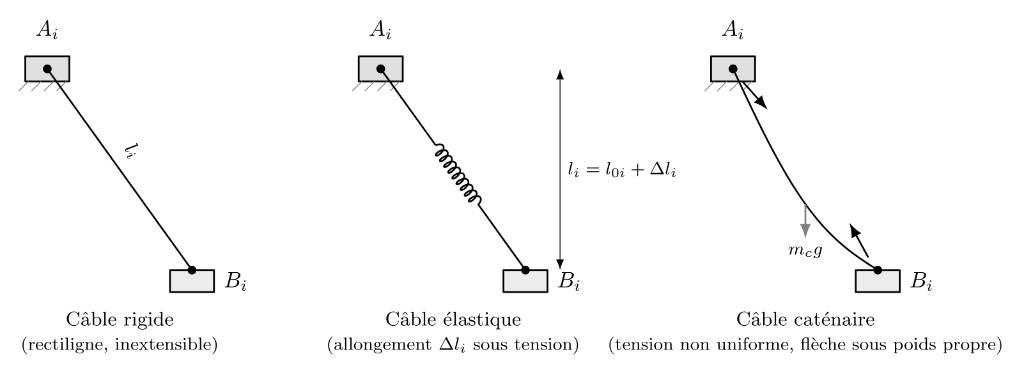
\includegraphics[width=0.95\textwidth]{cable_models.jpg}
\caption{Les trois modèles de câble : rigide, élastique, caténaire}
\label{fig:modeles_cable}
\end{figure}

\subsection{Câble rigide}

Le modèle de câble rigide est le plus simple. Il repose sur trois hypothèses :
\begin{itemize}
\item Le câble est sans masse ;
\item Il est inextensible, c'est-à-dire de raideur infinie ;
\item Il reste rectiligne entre ses deux points d'attache.
\end{itemize}
Dans ce modèle, la longueur du câble est directement donnée par la distance euclidienne entre le point d'ancrage fixe $A_i$ et le point d'attache mobile $B_i$ : aucune déformation ni affaissement n'est pris en compte. Ce modèle convient bien aux robots de petite taille dont les câbles sont courts et légers, et lorsque les tensions restent suffisamment élevées pour que l'élasticité et le poids propre soient négligeables. C'est aussi le modèle le plus utilisé pour la commande en temps réel, car il conduit à des calculs rapides et simples. C'est d'ailleurs celui adopté dans le modèle géométrique inverse de la section 1.2.

\subsection{Câble élastique}

Le modèle de câble élastique introduit la raideur axiale du câble. Il suppose que le câble reste rectiligne mais s'allonge proportionnellement à la tension appliquée, selon la loi de Hooke :
\begin{equation}
f_i = k_i (l_i - l_{0i})
\label{eq:hooke}
\end{equation}
où $l_i$ est la longueur actuelle du câble, $l_{0i}$ sa longueur à vide, et $k_i$ sa raideur axiale, donnée par :
\begin{equation}
k_i = \frac{E A}{l_{0i}}
\label{eq:ki}
\end{equation}
Avec $E$ : le module d'Young du matériau et $A$ la section du câble. Ce modèle est plus réaliste que le précédent dès lors que les câbles sont plus longs ou les charges plus importantes : il permet de prendre en compte l'allongement du câble sous tension, ce qui améliore la précision du positionnement. Il néglige en revanche toujours l'affaissement dû au poids propre du câble.

\subsection{Câble caténaire}

Le modèle de câble caténaire, le plus complet des trois, considère que le câble prend, sous l'effet de son propre poids, la forme d'une courbe caténaire entre ses deux points d'attache. La tension n'est alors plus uniforme le long du câble. Ce modèle se traduit par des équations non linéaires qui nécessitent une résolution numérique. Il devient indispensable pour les robots de grande envergure à câbles très longs, comme les robots FAST ou CoGiRo \cite{tho2022}, où l'affaissement n'est plus négligeable et affecte directement la précision de la pose. Pour de petites dimensions en revanche, son coût de calcul est généralement injustifié.

\section{Contraintes de tension}

La commande et la planification de trajectoire d'un robot parallèle à câbles (CDPR) sont conditionnées par le comportement mécanique des câbles eux-mêmes. Contrairement aux actionneurs rigides d'un robot série classique, un câble ne peut transmettre qu'un effort de traction. Cette spécificité impose deux contraintes qui doivent être respectées à tout instant et en tout point de la trajectoire : l'unilatéralité et les bornes de tension.

\subsection{Unilatéralité du câble}

Un câble ne peut exercer qu'un effort de traction ; il est incapable de pousser. La tension $f_i$ dans chacun des câbles doit donc rester strictement positive à tout instant :
\begin{equation}
f_i > 0 \qquad \text{(ou plus pratiquement } f_i \ge f_{\min}\text{)}
\label{eq:unilateralite}
\end{equation}
Cette contrainte, dite d'unilatéralité, constitue la condition fondamentale de faisabilité d'un CDPR \cite{tho2022}. Si la tension d'un câble s'annule, il se détend : la plateforme perd alors sa rigidité et le contrôle de sa pose n'est plus assuré, ce qui peut conduire à des oscillations, des imprécisions de positionnement, voire une instabilité du système.

En pratique, on n'exige pas seulement $f_i > 0$, mais $f_i \ge f_{\min}$, où $f_{\min}$ est une tension minimale de sécurité qui garantit que le câble reste tendu malgré les perturbations (vent, vibrations, imprécisions de mesure).

\subsection{Bornes de tension}

Si l'unilatéralité impose une borne inférieure, la résistance mécanique des câbles et la capacité des actionneurs imposent une borne supérieure. La tension dans chaque câble doit donc respecter l'intervalle suivant :
\begin{equation}
f_{\min} \le f_i \le f_{\max}
\label{eq:bornes}
\end{equation}
La borne inférieure $f_{\min}$ est fixée par la nécessité de maintenir tous les câbles tendus. Elle dépend de la précontrainte initiale, de la masse de la plateforme et des perturbations externes attendues.

La borne supérieure $f_{\max}$ est quant à elle déterminée par trois facteurs :
\begin{itemize}
\item La charge de rupture du câble, divisée par un facteur de sécurité ;
\item La capacité maximale des moteurs et des réducteurs, qui ne peuvent fournir qu'un couple limité ;
\item La déformation acceptable de la structure, le bâti ne devant pas fléchir sous l'effort.
\end{itemize}

Le respect simultané de ces bornes définit ce que la littérature appelle l'espace de travail en tension : l'ensemble des poses pour lesquelles il existe une distribution de tensions satisfaisant $f_{\min} \leq f_i \leq f_{\max}$ \cite{tho2022}.

Pour la planification : une trajectoire n'est réalisable que si, à chaque instant, les tensions calculées par la dynamique inverse restent dans l'intervalle admissible. Le non-respect de cette contrainte invalide la trajectoire, même si elle respecte par ailleurs les limites cinématiques des moteurs (vitesse, accélération).

\section{Espaces de travail}

La notion d'espace de travail est plus restrictive dans un robot parallèle à câbles que pour un robot rigide classique. En raison de l'unilatéralité des câbles et des bornes de tension, toutes les poses géométriquement atteignables ne sont pas nécessairement contrôlables. Duan et al. proposent une classification des espaces de travail fondée sur l'équation générale du mouvement et la propriété unilatérale des câbles \cite{duan2014}. Cette classification distingue cinq types d'espaces, dont trois sont particulièrement pertinents pour la planification de trajectoire.

\subsection{Espace de travail géométrique}

L'espace de travail géométrique est le plus large des espaces considérés. Il correspond à l'ensemble des poses pour lesquelles les longueurs de câbles calculées par le MGI (section 1.2) restent comprises entre les longueurs minimale et maximale admissibles, un câble ni totalement enroulé, ni totalement déroulé. Cet espace ne tient compte ni des tensions, ni de la gravité, ni de la capacité des moteurs : il fournit simplement une borne supérieure de l'espace réellement exploitable.

\subsection{Espace d'équilibre statique (SEW)}

L'espace d'équilibre statique (Static Equilibrium Workspace, SEW) est le sous-ensemble de l'espace géométrique dans lequel la plateforme peut être maintenue à l'arrêt, sous l'effet de la gravité, avec toutes les tensions positives \cite{duan2014}. Formellement, il existe un vecteur de tensions $\mathbf{f} > 0$ tel que :
\begin{equation}
\mathbf{J}^T \mathbf{f} + \mathbf{w}_g = \mathbf{0}
\label{eq:sew}
\end{equation}
où $\mathbf{J}^T$ est la matrice de structure transposée (section 1.2) et $\mathbf{w}_g$ le torseur de gravité. Le SEW est donc l'ensemble des poses où le robot peut tenir sa position sans bouger, mais il ne préjuge en rien de sa capacité à résister à des efforts externes.

\subsection{Espace de fermeture en effort (WCW)}

L'espace de fermeture en effort (Wrench Closure Workspace, WCW) est l'ensemble des poses pour lesquelles la plateforme peut équilibrer n'importe quel torseur d'effort : force et moment appliqué de l'extérieur, en tirant uniquement sur les câbles \cite{duan2014}. Autrement dit, quelle que soit la perturbation, il existe une distribution de tensions positives capable de la contrer. Le WCW est un espace très restrictif : il n'existe que pour les robots complètement contraints (au moins $n+1$ câbles pour $n$ degrés de liberté), et suppose qu'il n'y a aucune limite supérieure sur les tensions.

\subsection{Espace faisable en effort (WFW)}

L'espace faisable en effort (Wrench-Feasible Workspace, WFW) est le concept le plus pertinent pour la planification de trajectoire. Il correspond à l'ensemble des poses pour lesquelles la plateforme peut équilibrer un ensemble de torseurs d'effort prescrits, tout en gardant les tensions dans un intervalle borné :
\begin{equation}
f_{\min} \le f_i \le f_{\max}, \qquad \forall i \in \{1, \dots, m\}
\label{eq:wfw}
\end{equation}
Contrairement au WCW, le WFW prend en compte :
\begin{itemize}
\item La limite supérieure des tensions, liée à la capacité des moteurs et à la résistance des câbles ;
\item La limite inférieure, nécessaire au maintien de la tension pour éviter le mou (unilatéralité en section 1.4).
\end{itemize}
Le WFW constitue donc l'espace de travail réellement exploitable pour un CDPR. Une trajectoire n'est réalisable que si elle reste intégralement incluse dans le WFW. Son calcul dépend de la géométrie du robot, des bornes de tension et de l'ensemble des perturbations à contrer \cite{duan2014}.

Le tableau ci-dessous résume la hiérarchie des espaces de travail, du plus large au plus restrictif :

\begin{table}[H]
\centering
\caption{Synthèse comparative des espaces de travail}
\label{tab:espaces}
\resizebox{\textwidth}{!}{%
\begin{tabular}{|l|>{\raggedright\arraybackslash}p{3.6cm}|>{\raggedright\arraybackslash}p{3.0cm}|c|>{\raggedright\arraybackslash}p{3.0cm}|}
\hline
\textbf{Type d'espace} & \textbf{Condition} & \textbf{Limite de tension} & \textbf{Gravité} & \textbf{Utilisation} \\
\hline
Géométrique & Longueurs de câbles valides & Aucune & Non & Borne supérieure \\
\hline
SEW & $\mathbf{f} > 0$, équilibre statique & $f_i > 0$ & Oui & Pose de repos \\
\hline
WCW & Torseur quelconque équilibrable & $f_i > 0$ & Oui & Robots complètement contraints \\
\hline
WFW & Torseur prescrit équilibrable & $f_{\min} \leq f_i \leq f_{\max}$ & Oui & Planification de trajectoire \\
\hline
\end{tabular}%
}
\end{table}

\section*{Conclusion}

Ce chapitre a montré que la spécificité du CDPR, des câbles qui ne peuvent que tirer, impose des contraintes propres qui définissent en dernier ressort l'espace de travail réellement exploitable, le WFW. Cet espace, associé au modèle géométrique et à la représentation retenue de l'environnement, constitue désormais le cadre dans lequel toute trajectoire du robot Tandem devra s'inscrire. Il reste cependant à déterminer comment générer, à l'intérieur de ce cadre, un chemin couvrant la parcelle tout en conciliant rapidité, économie d'énergie et précision des prises de vue. C'est l'objet du chapitre suivant, consacré aux méthodes de planification et d'optimisation de trajectoire.

% ============================================================
% CHAPITRE 2 (début)
% ============================================================
